\section{Approach}
\label{sec:approach}

%\remark{D: Tom Funkhouser sold me on the value of this section, and one of the best examples from his papers is in http://www.cs.princeton.edu/~funk/pvg01.pdf. I actually like combining the Approach and Overview sections into one shorter section, though.}

%Restate the goal/problem. Use Sharon's more descriptive definition of a pattern template.
The goal of this paper is to develop a method for automatically generating pattern coloring suggestions to facilitate the creative coloring process. Although many people can easily detect if a pattern coloring is appealing, creating an appealing coloring can take much more time and effort. The process often involves much trial-and-error as well as tweaking of colors, due to constraints between neighboring regions. Since the relationship between neighboring colors largely impacts color appearance, changing one color also often results in cascading changes to neighboring colors. Even experienced artists create quick thumbnail colorings to explore potential color effects before diving in on their final work~\cite{ColorPaletteTools}. An effective color support system should output a wide variety of appealing colorings, as well as provide controls to let the user personalize suggestions to their preferred coloring style.

\remark{S: These are things I've read informally before and somewhat experienced, but citing more sources that describes these difficulties in the coloring process might be good. Similar statements on the coloring process would be nice in the introduction as well. Or, we can just mention this in the intro and then shorten the description here}

%Start of notes on pattern template terminology/definition.
Our approach takes as input a pattern template and any user-provided guidelines if available, and outputs suggested colorings for that pattern template. A pattern template specifies which regions in an image can be colored in, and which regions must map to the same color. For example, an image of a flower on a background may have a template that specifies all petals of the flower must be the same color, and all background regions must be the same color. In the rest of the paper, we refer to the set of regions that map to the same color as a \emph{color group}. Figure~\ref{fig:teaser} shows an example of a pattern template visualized in grayscale, where each different lightness level identifies a different color group. This pattern template representation is relatively easy to author from images composed of segments, such as web designs, renderings of 3D scenes, and line drawings. In this paper, we focus on 2D graphic design patterns. 

To generate attractive pattern colorings, a reasonable first step is to enforce that the colors used are `compatible' with one another, for some definition of color compatibility. Figure~\ref{fig:ColorCompatOnly} shows several patterns whose colors receive a high score under the color compatibility model of O'Donovan et al.~\shortcite{ODonovan}.~\remark{Make this figure.} While high-scoring colorings do exhibit a great degree of diversity, scoring a coloring based soley on the compatibility of its colors is not enough as pattern appearance also relies on relative proportion and spatial arrangement of colors. The colorings in the figure exhibit several problems due to arrangement, such foreground regions that blend into the background, and background regions that are too `loud' in color. Furthermore, color compatibility is a universal notion: it is not clear how to adapt it to match the style of a particular artist or the preferences of a particular user.

\begin{figure}
\centering
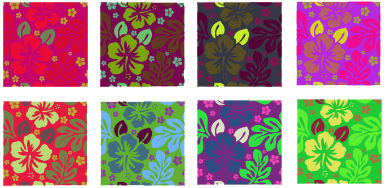
\includegraphics[width=\columnwidth]{figs/colorCompatOnly}
\caption{Patterns whose colors receive high scores under the color compatibility model of O'Donovan et al.~\shortcite{ODonovan}. Many patterns exhibit problems such as adjacent equi-luminant regions and excessively saturated backgrounds.~\remark{Figure not final.}}
\label{fig:ColorCompatOnly}
\end{figure}

%Large, background regions are colored differently than smaller, scattered `accent' regions; a thin, ribbon-like region against an empty field is colored differently than a thin region amidst a mass of similar regions.

%While compatible colors are an important component of attractive pattern colorings, they do not tell the whole story. The notion of color compatibility, whether implemented via the O'Donovan model or any other, considers colors abstractly: it does not take into account how they will be spatially used in the pattern. 

Rather than develop a specialized algorithm for this problem, we exploit the insight that both of these concerns---color harmony and spatial consistency---can be encoded in the extremely general framework of probabilistic factor graphs~\cite{FactorGraphs}. The framework allows us to leverage existing models of color compatibility. In the next section, we develop a data-driven factor graph model that can be trained on example colored patterns and sampled to generate new coloring suggestions. The factor graph formalism allows us to leverage existing models of color compatibility, to plug in additional coloring constraints in response to available user input, and to capture and inspect the characteristics of desired styles through established machine learning techniques.
